\begin{definition}[Image dataset]
	An image dataset in the scope of this thesis constists of input DIC images $X$ and target fluorescence images $Y$. Combined, couples from each form (X and Y) construct a dataset:
	\begin{equation}
		D = (X, Y) = \{(x^{(1)}, y^{(1)}), \dots, (x^{(N)}, y^{(N)})\}
	\end{equation}

	where both $x^{(i)}$ and $y^{(i)} \in \mathbb{R}^{W \times H}$ are single images, $N$ is the size of the dataset. Generally input data has a shape of $(N, C, H, W)$, in this work $C = 1$.
\end{definition}

\begin{definition}[Model]
	A model is a function with learnable parameters $\theta = (\theta_1, ..., \theta_K)$ where $\theta_i \in \mathbb{R}$ for $i \in {0, ..., K}$ which approximates the mapping of initial data $X$ to target data $Y$.
	\begin{equation}
		M(X,\theta) = Y^\prime \approx Y 
	\end{equation}
\end{definition}

\begin{definition}[Loss function]
	A loss function is a function $L(y, M(x, \theta))$ of model's parameters $\theta$, that for $(x^{(i)}, y^{(i)}) \in D$ outputs a scalar value measuring the difference between ground truth $y$ and prediction $M(x, \theta)$. A training objective is then defined as an average over the loss of each training sample:
	\begin{equation}
		J(\theta) = \mathbb{E}_{(x, y)\sim p_{data}} L(y, M(x, \theta))
	\end{equation}
	where $p_{data}$ denotes an empirical distribution of the training data.
\end{definition}

\begin{definition}[Weight initialization]
	Weight initialization is a process of setting the initial values of the parameters of a model to some random values.
\end{definition}

Weight initialization plays a crucial role in model training. Even on the simplest model wrongly initialized weights (for example all constant or too large or too small) can lead to very slow convergence or prevent the model from converging at all (\cite{Kumar_2017}).

In the following samples \textit{fan\_in} denotes the maximum number of input signal units to a given layer and \textit{fan\_out} is the maximum number of output signal units from it.

\begin{definition}[Xavier initialization]
	Xavier initialization, which is usually a default choice in many neural networks, works well for the most part for fully connected layers with tanh as activation function. There is also a study providing some insights into why Xavier initialization may not be the optimal choice for ReLU activations (\cite{Kumar_2017}). Xavier initialization draws samples from a uniform distribution:
	\begin{equation}
		Uniform \left(-\frac{1}{\sqrt{fan\_in}}, \frac{1}{\sqrt{fan\_in}}\right)
	\end{equation}
\end{definition}

\begin{definition}[He initialization]
	He initialization is another initialization method proposed by \cite{He_2015} as it was noticed that Xavier initialization is not an optimal choice for the networks that include ReLU activations. The authors suggest a new robust method that enables training of even extremely deep or wide network architectures with ReLU activations. He initialization draws samples from a truncated normal distribution:
	\begin{equation}
		N(0, \sqrt{\frac{2}{\text{fan\_in}}})
	\end{equation}
\end{definition}

Default weight initialization of Conv2D layers in Python suggests to use the following initialization method (\cite{He_2015}):
\begin{align}
	std &= \sqrt{\frac{2}{fan\_in}} \\
	bou&nd = \sqrt{3 * std} \\
	Un&iform\left(-bound, bound\right)
\end{align}

Although in the study of \cite{He_2015} it is called Kaiming normal initialization, it is a slightly different method.

\begin{definition}[Binary-cross entropy loss]
	Let $y \in \mathbb{R}^{W \times H}$ be a ground truth image and $y^\prime \in \mathbb{R}^{W \times H}$ be a prediction. Binary-cross entropy loss is defined as:
	\begin{equation}
		L(y, y^\prime) = - \frac{1}{N^2}\sum_{i=1}^{H} \sum_{j=1}^{W} y_{i,j} \cdot \log(y_{i, j}^\prime) +  (1 - y_{i, j}) \cdot \log(1 - y_{i, j}^\prime) 
	\end{equation}
\end{definition}

\begin{definition}[MSE (mean squared error) loss]
	Let $y \in \mathbb{R}^{W \times H}$ be the ground truth and $y^\prime \in \mathbb{R}^{W \times H}$ be the predicted images. The MSE loss is defined as:
	\begin{equation}
		L(y, y^\prime) = \sum_{i=1}^{H} \sum_{j=1}^{W} (y_{i, j} - y_{i, j}^\prime)^2
	\end{equation}
\end{definition}

\begin{definition}[PCC (Pearson correlation coefficient) loss]
	\label{def:pcc-loss}
	Let $y \in \mathbb{R}^{WH}$ be a flattened ground truth and $y^\prime \in \mathbb{R}^{WH}$ be a flattened predicted image. The PCC loss is defined as:
	\begin{align}
		PCC(y, y^\prime) &= \frac{\sum_{i=1}^{{WH}}{(y_i - \bar{y})(y_i^\prime - \bar{y}^\prime)}}{\sqrt{\sum_{i=1}^{{WH}^2}{(y_i - \bar{y})^2(y_i^\prime - \bar{y}^\prime)^2}}}  \\
		L(y, y^\prime) &= \frac{1 - PCC(y, y^\prime)}{2}
	\end{align}
	where $\bar{y}$, $\bar{y}^\prime$ are means of the ground truth and predicted images respectively.
	
	There is an important distinction to be made here: firstly, Pearson correlation coefficient (PCC further) in a measure of similarity between two data sequences (matrices in this case), with values between $-1$ and $1$, with $1$ being a positive correlation, secondly, PCC loss is a measure of dissimilarity between two matrices, with values between $0$ and $1$, with $0$ meaning that matrices are the same.

	This loss is widely used in cell biology for comparison of co-localization between the proteins (\cite{Lachance_2020}). PCC is also popular in computer vision where it is utilized for the determination of image similarity in terms of spatial-intensity (\cite{Lachance_2020}).
\end{definition}

\begin{definition}[Optimization]
	Optimization is a process of updating the parameters $\theta$ of the model $M(X, \theta)$ to minimize the loss function $L(y, M(x, \theta))$.
\end{definition}

With a maximum likelihood esimation, we get:
\begin{equation}
	\theta_{MLE} = \argmax\limits_{\theta} \sum_{i=1}^{N} \log{p_{\text{model}}(x^{(i)}, y^{(i)}, \theta)}
\end{equation}

After maximizing the sum and taking a gradient one gets:
\begin{equation}
	\nabla_{\theta} J(\theta) = \mathbb{E}_{x, y \sim p_{data}} \nabla_{\theta} \log{p_{\text{model}}(x, y, \theta)}
\end{equation}

The exact gradient on a discretized data-generating distribution is then:
\begin{equation}
	g = \nabla_{\theta} J^*(\theta) = \sum_{x} \sum_{y}{p_{\text{data}}(x, y) \nabla_{\theta} L(y, M(x, \theta))}
\end{equation}

Here one can obtain an unbiased estimator of a true gradient on a mini-batch of i.i.d. samples $\{x^{(i)}, ..., x^{(m)}\}$	

\begin{equation}
	\hat{g} = \frac{1}{m} \nabla_\theta \sum_{i} L(y^{(i)}, M(x^{(i)}, \theta))
\end{equation}

\begin{definition}[Stochastic gradient descent]
	Stochastic gradient descent is an optimization algorithm where the parameters $\theta$ are iteratively updated every mini-batch of data by the following rule:
	\begin{equation}
		\theta_{k+1} = \theta_k - \alpha \frac{1}{m} \nabla_\theta \sum_{i} L(y^{(i)}, M(x^{(i)}, \theta))
	\end{equation}
	where $\alpha$ is a tuneable parameter called \textit {learning rate}.
\end{definition}

\begin{definition}[Adadelta optimizer]
	An Adadelta optimizer is a more sophisticated optimization technique, that follows algorithm \ref{alg:adadelta} for the parameter update.
	\begin{algorithm}[H]
		\caption{Adadelta optimization}\label{alg:adadelta}
		\item 1. $E[g]^2_0 = 0$ and $E[\Delta \theta^2]_0 = 0$
		In order to update the parameters one needs to:
		\item 2. Compute gradient: $g_t$
		\item 3. Accumulate gradient: $E[g]^2_t = \rho E[g]^2_{t - 1} + (1 - \rho)g_t^2$
		\item 4. Compute update: $\Delta \theta_t = \frac{\text{RMS}[\Delta \theta]_{t-1}}{\text{RMS}[g]_t} \hat{g_t}$
		\item 5. Accumulate updates: $E[\Delta \theta^2]_t = \rho E[\Delta \theta^2]_{t-1} + (1 - \rho) \Delta \theta^2_t$
		\item 6. Apply update: $\theta_{t+1} = \theta_t + \Delta \theta_t$ \\
		RMS here is the root mean square all initial hyperparametes are take from the original study(\cite{Zeiler_2012}).
	\end{algorithm}
\end{definition}

\begin{definition}[Adam optimizer]
	An Adam optimizer is another stohastic optimization technique, that has the following hyperparameters: $\alpha$ --- learning rate, $\beta_1, \beta_2 \in [0, 1)$ --- exponential decay rates. It follows algorithm \ref{alg:adam} for the parameter update.
	\begin{algorithm}[H]
		\caption{Adam optimization}\label{alg:adam}
		\item 1. Initialize: $m_0 = 0$ and $v_0 = 0$
		\item 2. Compute gradient: $g_t$
		\item 3. Update biased first moment estimate: $m_t = \beta_1 m_{t-1} + (1 - \beta_1) g_t$
		\item 4. Update biased second raw moment estimate: $v_t = \beta_2 v_{t-1} + (1 - \beta_2) g_t^2$
		\item 5. Compute bias corrected first moment estimate: $\hat{m_t} = \frac{m_t}{1 - \beta_1^t}$
		\item 6. Compute bias corrected second raw moment estimate: $\hat{v_t} = \frac{v_t}{1 - \beta_2^t}$
		\item 7. Apply update: $\theta_{t+1} = \theta_t - \alpha \frac{\hat{m_t}}{\sqrt{\hat{v_t} + \epsilon}}$
		Initial hyperparameters used in this work are $\alpha = 0.001$, $\beta_1 = 0.9$, $\beta_2 = 0.999$ and $\epsilon = 10^{-8}$.
	\end{algorithm}
\end{definition}

\begin{definition}[Overfitting]
	Overfitting is a phenomenon in which a hypothesis that fits training samples well will perform worse over the entire distribution on data rather than another hypothesis that fits the distribution of the training samples less well (\cite{mitchell_1997}). The way to avoid overfitting that happened to the models in Section \ref{section:er} are discussed in Section \ref{section:regularization}.
\end{definition}

\begin{definition}[Feedforward fully connected layer]
	A feedforward fully connected layer is a trainable function with parameters $W \in \mathbb{R}^{N \times M}$ (weights) and $b \in \mathbb{R}^{M}$ (biases) that, in this case, maps a vector $x \in \mathbb{R}^{N}$ to an output $a \in \mathbb{R}^{M}$ via the following transformation:
		\begin{equation}
			a = W^{T}x + b
		\end{equation}
\end{definition}

This is one of the simplest layers in a feedforward neural networks and input and output in it as mentioned above are vectors. However, in this study inputs and outputs are images, that are represented in memory as square matrices $x^{(i)}, y^{(i)} \in \mathbb{R}^{N \times N}$. One could simply flatten the image into a vector and use it as an input to a fully connected feedforward neural network. Nevertheless this would be a suboptimal approach. 

Since essentially one of the main tasks of this research is to create a deep learning model that is able to predict a fluorescence image from a DIC image, the problem statement could be narrowed down to the following: predict an intensity high-resolution image from another intensity high-resolution image based on the features of the object morphology in it. Such problem is very common in the field of image analysis and one of the popular deep learning tools for solving such problems is convolutional neural network (CNN) or more specifically a UNet.

CNNs are able to capture nonlinear relationships over large areas of images, they greatly improve performance for image recognition tasks in comparison to classical machine learning methods (\cite{Ounkomol_2018}). The word "convolutional" suggests that the convolution operation should be used in at least one of the layers there.  

\begin{definition}[Convolutional layer]
	A convolutional layer is a trainable function with parametrized kernel $K \in \mathbb{R}^{F \times F \times C}$ and bias $b \in \mathbb{R}$ that is usually denoted via the operator $(\cdot * \cdot)$. By transforming an input $x \in \mathbb{R}^{W \times H \times C}$ it produces an output $S$
	\begin{equation}
		S = K * x + b
	\end{equation}

	that is called a \textit{feature map} where an element on position $(i, j)$ is defined as follows:
		\begin{equation}
			S_{i, j} = \sum_{w} \sum_{h} x_{m, n}  K_{i - m, j - n}
		\end{equation}
\end{definition}

Convolutional layer like a fully connected layer can be viewed a linear transformation as well. However, there are three main advantages that leverage convolutional layers for image processing in comparison to fully connected layers: sparse interactions, parameter sharing and equivariant representations. An image is a very redundant way of representing the semantic meaning hidden within it. Having a value of one pixel, the probability that the neighboring one will be of the same color is very high. Sparsity of interactions can be described by an example: usually a high-resolution image might have millions of pixels, however it is possible to detect smaller and very important features like contrast changes, edges, and shapes using a kernel consisting of only a few hundred pixels. By applying kernels (or filters) on the image locally, one will infer many of these features across the whole image. Such an approach reduces the memory needed for parameter storing and improves its statistical efficiency (\cite{Goodfellow_2016}). Parameter sharing refers to the fact that instead of learning a separate set of parameters for every location within the image, only one set of parameters will be learned and applied across all image locations. Lastly, equivariance here means that convolution operation is equivarient to the shifts in the image.

\begin{definition}[Stride]
	During the computation of convolution, the kernel starts sliding at the upper left corner of the input tensor, covering all locations while heading to the right and down. The step with which the window slides is called \textit{stride}. 
\end{definition}

\begin{definition}[Padding]
	When convolution is applied several points on the perimeter of the input tensor will be lost and the ouput tensor will have smaller spatial dimension than the input one. One can fix this by adding a few more pixels outside the perimeter, to preserve the dimension of the output to be same as input. The amount of pixels added is called \textit{padding}. 
\end{definition}

Visual examples of what stride and padding represent are shown in Figure \ref{fig:stride}.
\begin{figure}[htb]
	\begin{center}
		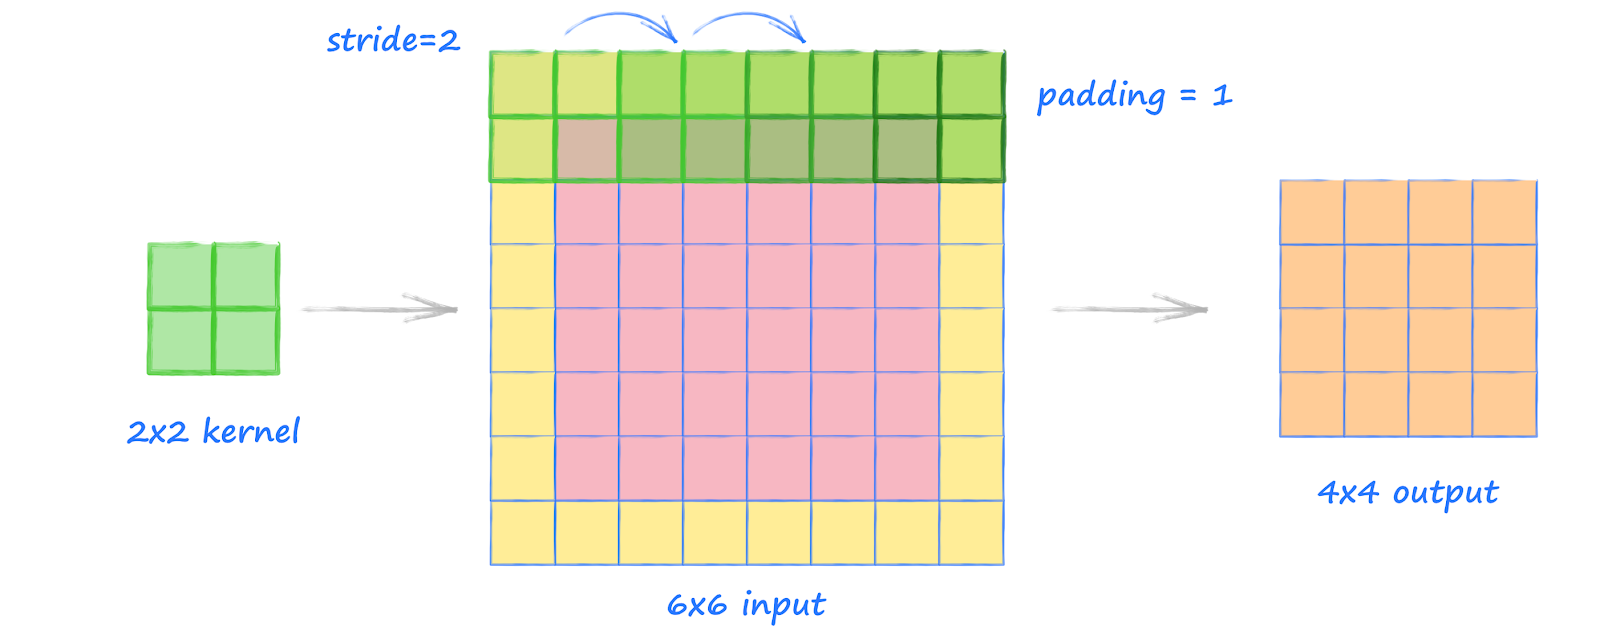
\includegraphics[width=0.6\linewidth]{bilder/stride_padding.png}
		\caption[Stride and padding example]%
		{Stride and padding example. Taken from \cite{stride}.}
		\label{fig:stride}
	\end{center}
\end{figure}

\begin{definition}[Max-pooling layer]
	Maximum pooling operation reports the maximum output within a rectangular neighborhood (\cite{Goodfellow_2016}).
\end{definition}

\begin{definition}[Activation function]
	An activation function is an element-wise non-linear function $f(\cdot)$. Some examples are:
	\begin{align}             
		f(x) = \frac{1}{1 + e^{-x}} &&\text{Sigmoid} \\      
		f(x) = max(0, x) &&\text{Rectified linear unit (ReLU)}\\
		f(x) = \begin{cases}
				x, \hspace*{1cm} \textrm{if } x > 0 \\
				\alpha * (e^{x} - 1), \textrm{if }  x \leq 0
		  	\end{cases}\ &&\text{ELU}
		\end{align}
\end{definition}

It is important to use activation functions after each convolutional or linear layer like RELU, ELU, Tahn, Sigmoid or any other non-linearities. Because any combination of linear functions can be represented with another linear function, having consecutive linear layers without non-linear function in the network is equivalent to having just one linear layer. Non-linearities  In CNNs they are also often combined with max-pooling layers and dropouts to escape overfitting. 

\begin{definition}[Batch normalization layer]
	Let's denote $B = \{x^{(i)}, ..., x^{(m)}\}$ to be a mini-batch of data. Then batch normalizing transform applied to this input data would be:
	\begin{equation}
		\begin{split}
		& a^{(i)} = \gamma \frac{x^{(i)} - \mu_B}{\sigma^2_B + \epsilon} + \beta \\
		& \sigma^2_B = \frac{1}{m} \sum_i^m (x^{(i)} - \mu_B)^2 \\
		& \mu_B = \frac{1}{m} \sum_i^m x^{(i)} \\
		\end{split}
	\end{equation}
	where $\gamma$ and $\beta$ are learnable parameters, $\mu_B$ and $\sigma^2_B$ are the mean and standard deviation of the batch (\cite{Ioffe_2015}).
\end{definition}

\begin{definition}[Dropout layer]
	Dropout is a technique that randomly sets some weights (units) to zero (\cite{Srivastava_2014}). It leads to the training of several smaller networks that share the parameters. If a mask vector $\mu$ specifies which units are included in training, then dropout's objective to be minimized becomes: $\mathbb{E}_\mu J(\theta, \mu)$. Visually dropout is presented in the Figure \ref{fig:dropout}.
\end{definition}

%TODO add figure reference!
\begin{figure}[H]
	\begin{center}
		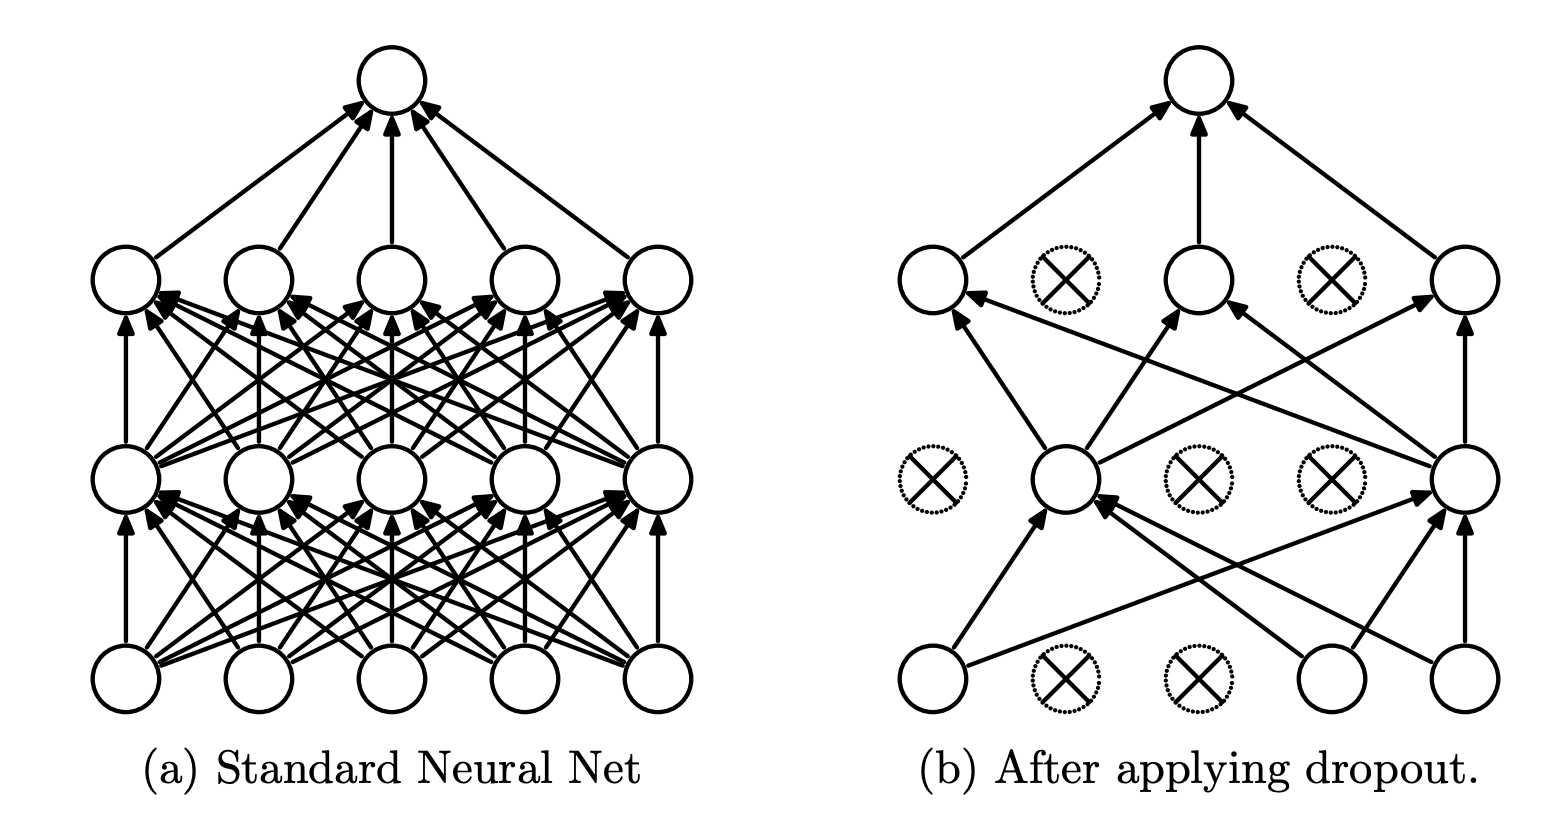
\includegraphics[width=0.5\linewidth]{bilder/dropout.png}
		\caption[Dropout]%
		{Dropout. Taken from \cite{Srivastava_2014}}
		\label{fig:dropout}
	\end{center}
\end{figure}

The models in this project mostly use ELU activations as ELU provides a better signal flow between the layers by not cutting off the negative values completely.

\begin{definition}[UNet]
	UNet is fully convolutional neural network with U-shaped encoder-decoder network architecture (\cite{Ronneberger_2015}). Example of the UNet architecture can be found in Figure \ref{fig:unet}.
\end{definition}

The encoder is a common CNN, consisting of the repeated
block of two $3 \times 3$ convolutions, followed by
an activation function, and a $2 \times 2$ max-pooling operation with stride 2. At each encoder step  the number of feature channels doubles. The decoder is also a CNN, consisting of repeated blocks of transposed convolution, that halves the number of feature channels, followed by a concatenation with a corresponding output from an encoder, and two $3 \times 3$ convolutions, followed by a ReLU. The last decoder layer is a $1 \times 1$ convolution to map the tensor to the number of output image channels needed. Skip-connections is a very important part of UNet as they allow to the flow of high-resolution features from the encoder to the decoder that in turn allows to restore a corresponding high-resolution image.

\begin{definition}[Autoencoder]
	Autoencoder is an unsupervised learning technique in neural networks for the representation learning purposes. Autoencoder consists of an encoder that compresses data into a lower dimensional representation and a decoder that restores the original input from the encoded representation.
\end{definition}

\paragraph{Regularization techniques}
\label{section:regularization-theory}
% TODO add overfitting image?
Regularization is mostly used to prevent a deep learning model to overfitting on the training data and to be able to generalize well. Overfitting has occured in the models used in this research and therefore it is improtant to understand the techniques that can be used to prevent it. There are are several approaches to regularize the model and they will be explained below.

\begin{itemize}
	\item Early-stopping

	Overfitting can be detected via visualizing train and validation losses. Training behaviour at first will be the usual one, meaning that both train and validation losses are gradually decreasing, however at some point the train loss continues to decrease, whereas the validation loss suddenly starts to increase. Since the model has not seen any of the data from the validation set, it means that it loses its ability to generalize on unseen data, while improving its perfomance on the seen data (train set). This does not happen during earlier epochs. Assuming that the model learns a complex decision surface while training, the weights of the model will be quite small and random with the correct weight initialization and therefore the best decision surface during the early epochs would be a smooth one. But during the later ones the difference in values of the weights grows and they become dissimilar which also means that the decision surface becomes more complex and the model is now able to fit not only the training data itself, but also its noise (\cite{mitchell_1997} p.111). And that is why stopping before the model becomes too complex, meaning to stop before the overfitting point, mitigates this problem.

	\item \emph{L1}- \emph{L2}-regularization

	The complexity of the deep model grows with the number of features it uses, sometimes the model may pay attention to the features that are not important to the outcome, or even considers noise to be a feature. To prevent this one should decrease the weights associated with useless features, however one cannot know ahead of time which of them should be ignored, therefore one may limit them all (\cite{Ying_2019}). In order to do that, a penalty term is added to the loss function:

	\begin{equation}
	\tilde{L}(Y, M(X, \theta)) = L(Y, M(X, \theta)) + \lambda R(\theta)
	\end{equation}

	for some $\lambda > 0$. This is called a \emph{soft-constraint} optimization. When $R(\theta)$ is of the form $R(\theta) = ||\theta||^2_2 = \sqrt{\sum\limits_i \theta_i^2}$ this is called \emph{L2}-regularization. When it is of form $R(\theta) = ||\theta||_1 = \sum\limits_i |\theta_i|$ this is called \emph{L1}-regularization. \emph{L2}-regularization used in combination with backpropagation is equivalent to weight decay. Weight decay is defined by \cite{Hanson_1988} as follows:
	\begin{equation}
		\theta_{t+1} = (1 - \lambda)\theta_t - \alpha \frac{\partial L}{\partial \theta_t}
	\end{equation}

	where $\alpha$ is a learning rate. Weight decay successfully has more effect on the weights along which the gradient change is smaller \cite{Goodfellow_2016}. \emph{L1}-regularization induces sparsity of the weights by assigning some of them to zero, this could also be considered as a feature selection approach.

	\item Regularization layers

	Batch normalization and dropout layers are also considered to be a form of regularization.

	\item Network reduction

	Since learning a too complex and noise-fitting decision surface might be a frequent cause of an overfit, another way to mitigate this would to be reduce the space of the possible decision surfaces and therefore make the surface simpler so that it cannot fit into the noise from the data. By changing the number of adaptive parameters in the network, the complexity can be varied (\cite{Bishop_2006} p.332).

	\item Expansion of the training data

	For a successful training a model needs to have a sufficient amount of quality samples. An expanded dataset can improve the quality of the predictions \cite{Ying_2019}, however only when the model has already performed well on the initial dataset. If the model was performing badly initially, adding more data will not solve the problem.
\end{itemize}
